The wage gap is an oft-cited number of the differences between males' and females' adult outcomes: In the fourth quarter of 2016, white women earned 81.1\% as much as white men and black women earned 92.1\% as much as black men. This reveals a gap not only by gender, but also by race with Black (Hispanic) women only earning 67.8\% (62.0\%) as much as white men and black (Hispanic) men earning 73.6\% (71.4\%) as much as white men.\footnote{\citet{USDPTL_2017_Wage_News-Release}.}

 Although this favors males, there are related measures of gender differences that favor females. In both criminal activity and educational attainment, females fare better than males, on average. In 2015, 488 per 100,000 males were incarcerated in comparison to 64 per 100,000 females. When further dividing these statistics by race, the difference between genders and races becomes more stark. While 457 per 100,000 white males were incarcerated, 2,613 (1,043) per 100,000 African-American (Hispanic) males were incarcerated. The rates for females were 52 per 100,000 white females in comparison to 103 (63) per 100,000 African-American (Hispanic) females.\footnote{\citet{UDOJ_2016_PrisonersStatistics_Bulletin}.} In 2012-2013, more females than males received bachelor's degrees across all races with larger disparities for African-American (65\% of the degrees conferred to females) and Hispanics (60\%).\footnote{\citet{UDOE_2016_Statistics_Report}.}

These differences are static measurements from the life-cycle trajectory of skill formation and labor market opportunities. Based on the work of human capital formation, these later skills build on earlier skill development.\footnote{\citet{}.} Additionally, higher levels of these skills, especially social-emotional skills, can lead to more positive life-relevant outcomes, such as increased employment.\footnote{\citet{}.} Adult differences between males and females can be the result of early-life differences developing over the life-cycle. We examine these early-life gender differences and their evolution over the life-cycle by analyzing the effects of two nearly identical early childhood interventions. 

The interventions, the Carolina Abecedarian Project (ABC) and the Carolina Approach to Responsive Education (CARE), were randomly offered to disadvantaged families in Chapel Hill, North Carolina with children born between 1977 and 1980. The treatment group received received high-quality, intensive, early childhood education from shortly after birth until entrance into elementary school. Researchers collected measures of cognitive, social-emotional, and parenting skills on the children in both the treatment and control groups during and after treatment. 

Using the ABC/CARE sample and pooling across experimental groups, Figure~\ref{fig:intro-skills-plots} shows the skill differences between the males and females. Consistent with previous work, females tend to perform better in early skill measurements, although this is only precisely the case for social-emotional skills in this case.\footnote{\citet{}.} The parenting shows more mixed results with parents of males exhibiting more positive parenting skills than those of females during later ages (3.5, 4.5, and 8 years), but mothers of females showing more warmth and involvement than those of males.

\begin{sidewaysfigure}[H]
\begin{center}
\caption{Differences Between ABC/CARE Males and Females, Skill Measurements}
\label{fig:intro-skills-plots}
\begin{subfigure}[b]{0.49\textwidth}
	\caption{IQ Measurements}
	\label{fig:intro-skills-plots-cog}
	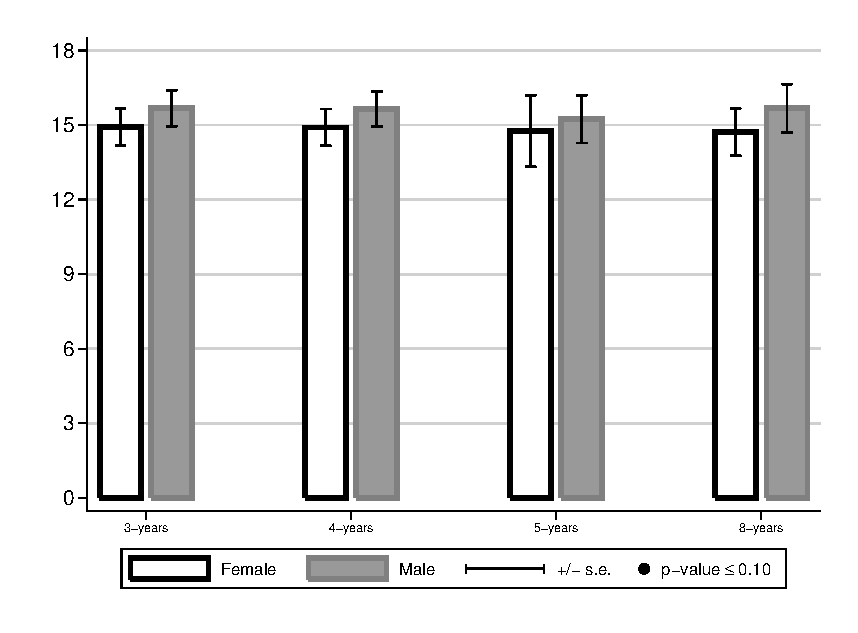
\includegraphics[width=\textwidth]{../output/abccare-gdiff-cog}
\end{subfigure}
\begin{subfigure}[b]{0.49\textwidth}
	\caption{Social-emotional Measurements}
	\label{fig:intro-skills-plots-ncog}
	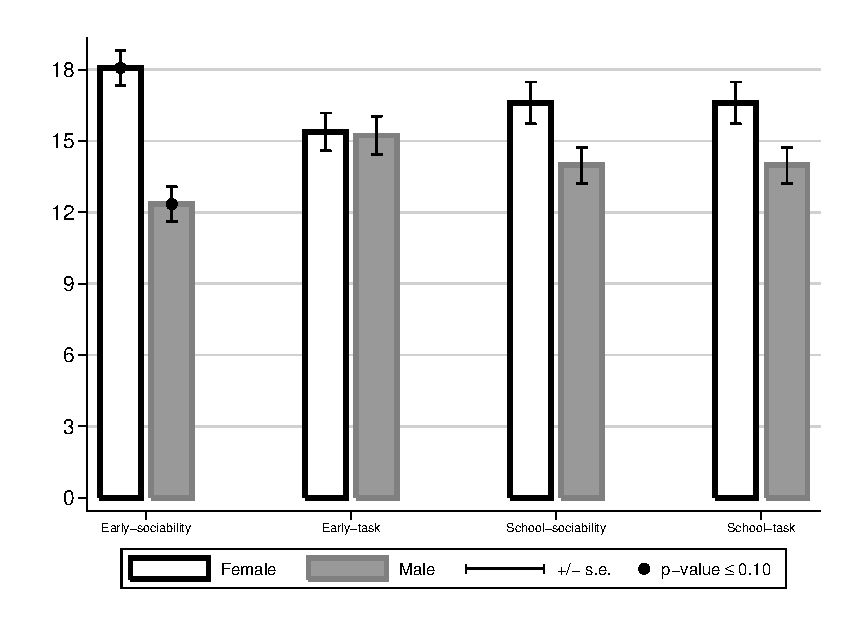
\includegraphics[width=\textwidth]{../output/abccare-gdiff-ncog}
\end{subfigure}

\begin{subfigure}[b]{0.49\textwidth}
	\caption{Achievement Measurements}
	\label{fig:intro-skills-plots-ach}
	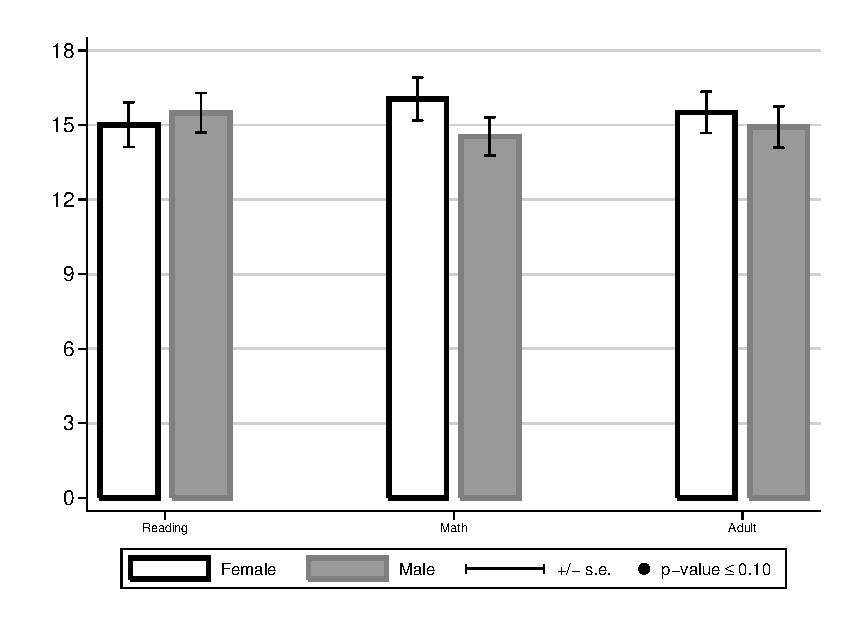
\includegraphics[width=\textwidth]{../output/abccare-gdiff-ach}
\end{subfigure}
\begin{subfigure}[b]{0.49\textwidth}
	\caption{Parenting Measurements}
	\label{fig:intro-skills-plots-parenting}
	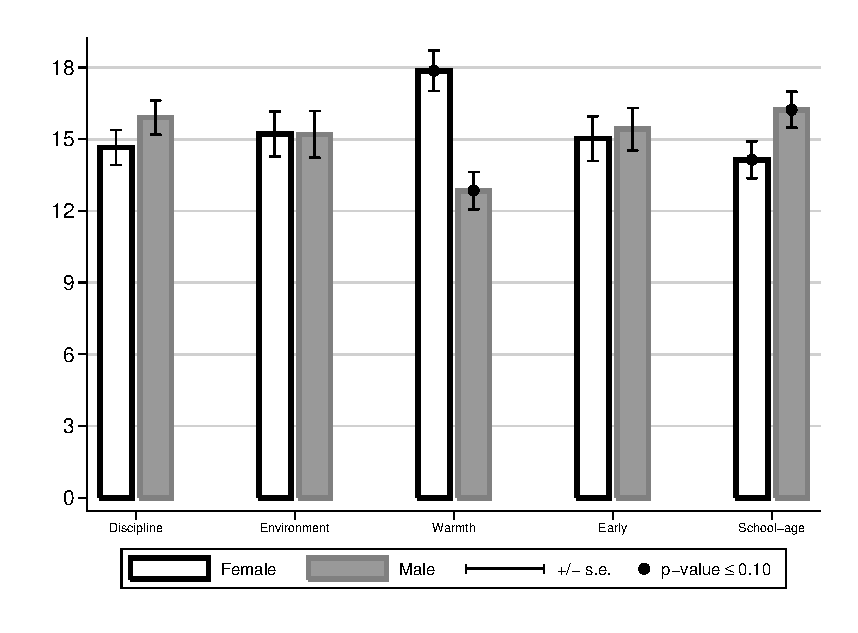
\includegraphics[width=\textwidth]{../output/abccare-gdiff-parenting}
\end{subfigure}
\end{center}
\raggedright \scriptsize
Note: These plots show the means of factor variables by gender, pooling across experimental groups. The capped lines show the standard errors and black points indicate that the female is significantly different than the males. These hypothesis tests are one-sided and computed using 200 bootstraps. All factor variables are calculated by principal factor analysis. The factors are then standardized and divided into 30 quantiles. The IQ factors include different measurements at the specified ages. The social-emotional factors are divided by early (0.5, 1, and 1.5 years) and school-age (6 and 8 years). The scales presented here are sociability and task orientation. The achievement factors are school-age math and reading factors (6, 7.5, 8, 8.5, 9, and 12 years) and an adult factor combining math and reading at 21 years. The parenting factors include factors of the subscales absence of punishment (discipline), environmental factors (environment), and maternal warmth and involvement (warmth). The other factors combine these scales measured when the subjects were toddlers (0.5, 1.5, and 2.5 years) and when they were older (3.5, 4.5, and 8 years).
\end{sidewaysfigure}

We can also examine the gender differences in adult outcomes. As shown in Figure~\ref{fig:intro-adult-outcomes}, females commit fewer crimes, but have worse health and lower education and income levels. Although females do better on average than males early in life, they lag behind males later in life in important outcomes.

\begin{figure}[H]
\begin{center}
\caption{Differences Between ABC/CARE Males and Females, Adult Outcomes}
\label{fig:intro-adult-outcomes}
	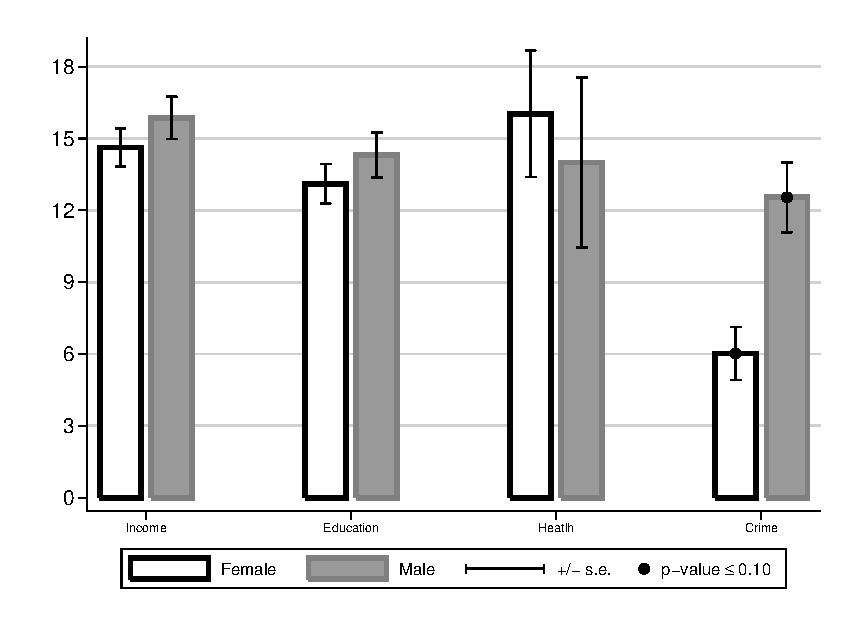
\includegraphics[width=0.9\textwidth]{../output/abccare-gdiff-adult}
\end{center}
\raggedright \scriptsize
Note: This plot shows the means of factor variables by gender, pooling across experimental groups. The capped lines show the standard errors and black points indicate that the female is significantly different than the males. These hypothesis tests are one-sided and computed using 200 bootstraps. All factor variables are calculated by principal factor analysis. The factors are then standardized and divided into 30 quantiles. The income factor is comprised of income labor at 21 and 30 years and employment at 30 years. The education factor is comprised of years of education and college graduation at 30 years and high school graduation at 21 years. The health factor is coded such that a higher value corresponds to socially undesirable outcomes. It is comprised of measures of drug and tobacco use, obesity, and hypertension. The crime factor is comprised of total felony and misdemeanor arrests using administrative data collected when the subjects were in their mid-30s.
\end{figure}

Although these mean differences do not include the effect of the early childhood education on improving these skills, many studies have shown the potential for early-life interventions to improve the skills of children, especially those from disadvantaged families.\footnote{\citet{Elango_Hojman_etal_2016_Early-Edu}.} Several of these studies separate analysis by gender and find that males and females benefit differently from early childhood education. For example, \citet{Heckman_Moon_etal_2010_QE} and \citet{Garcia_etal_2016_Comp_CBA_Unpublished}, both of which analyze randomized controlled trials with long-term data follow-ups, find that females tend to have more positive effects in education outcomes while males tend to have more positive effects in labor market and health outcomes. Other studies analyzing programs with shorter-term data also find gender differences in early skills and academic outcomes.\footnote{\citet{Deming_2009_AEJAE} and \citet{Ou_Reynolds_2010_Mechanisms_CYSR} are examples of this.} 

There are several explanations for these early differences. One supported in neurobiology is that males are more fragile than females early in life.\footnote{\citet{}.} Another explanation from psychology is that parents respond differently by gender while the children are developing and learning.\footnote{\citet{}.} We explore these potential mechanisms and others.

We describe ABC/CARE in more detail in Section~\ref{sec:data}. We then discuss the parameters of interest in Section~\ref{sec:parameters} and describe our method for summarizing over the variables in Section~\ref{sec:combining-functions}. Section~\ref{sec:treatment-effects} displays the estimates from both of these methods. We discuss suggestive mechanisms through which the early-life skill differences mediate later-life gender differences in Section~\ref{sec:gender-differences}. Section~\ref{sec:conclusion} concludes.

%These gender results are variable across studies, however, obfuscating the conclusions.\footnote{\citet{Magnuson_Kelchen_Duncan_etal_2016_ECRQ} use effect sizes and program characteristics from 23 evaluations of early-life interventions to understand the association between program characteristics and effect sizes by gender. This meta-analysis finds that over the programs used, the most pronounced difference in treatment effects between males and females can be found for outcomes related to schooling, e.g. special education and grade retention. However, most of the programs do not have non-cognitive measures and the varied structure of the evaluations makes the conclusions for gender differences suggestive.} Even within the same program, different approaches to analyzing treatment effects can result in seemingly contradictory conclusions. Using data from the Carolina Abecedarian Project and the Carolina Approach to Responsive Education (ABC/CARE), \citet{Garcia_etal_2016_Comp_CBA_Unpublished} calculate a higher lifetime benefit-cost ratio for males (11.10) than for females (2.45), with these ratios including life-cycle projections of health, crime, and income. According to this analysis, the monetary returns of the program from a social perspective are driven more by males than females, making it appear that males benefit more from the program than do females. However, when looking at the treatment effects unweighted by monetary amounts, there are more positive treatment effects for females for certain categories (see Section~\ref{sec:gdiff}). Unlike the cost-benefit analysis, this aggregate result makes it appear that females benefit more from the program in skills, labor market outcomes, and crime outcomes. Although both of these measures aggregate across outcomes, they lead to seemingly contradictory conclusions on the differential effect of early childhood education.

%Understanding the mechanisms of the treatment effects complements the above analyses by explaining and understanding the later-life gender differences seen in both approaches. We address the contradiction by focusing on how early childhood education affects the skill formation process of males and females differently, with these skills in turn affecting other outcomes.\footnote{There is also evidence that the development of males and females differs at this age such that they experience early childhood interventions differently. See \citet{Beeghly-etal_2017_IMHJ,Dayton_2017_IMHJ,Iruka_2017_IMHJ,Schore_2017_IMHJ} for recent findings on the topic of different development of males and females early in life. We consider these findings complementary to our own.}

